\documentclass[10pt]{beamer}

\usetheme{metropolis}
\usepackage{appendixnumberbeamer}

\usepackage{booktabs}
\usepackage[scale=2]{ccicons}

\usepackage{pgfplots}
\usepgfplotslibrary{dateplot}

\usepackage{xspace}
\newcommand{\themename}{\textbf{\textsc{metropolis}}\xspace}
\setbeamertemplate{frame footer}{ME738 - Special Topics in Materials}

\title{}
\subtitle{}
% \date{\today}
\date{February 1, 2024}
\author{Tommaso Bocchietti}
\institute{University of Waterloo}
% \titlegraphic{\hfill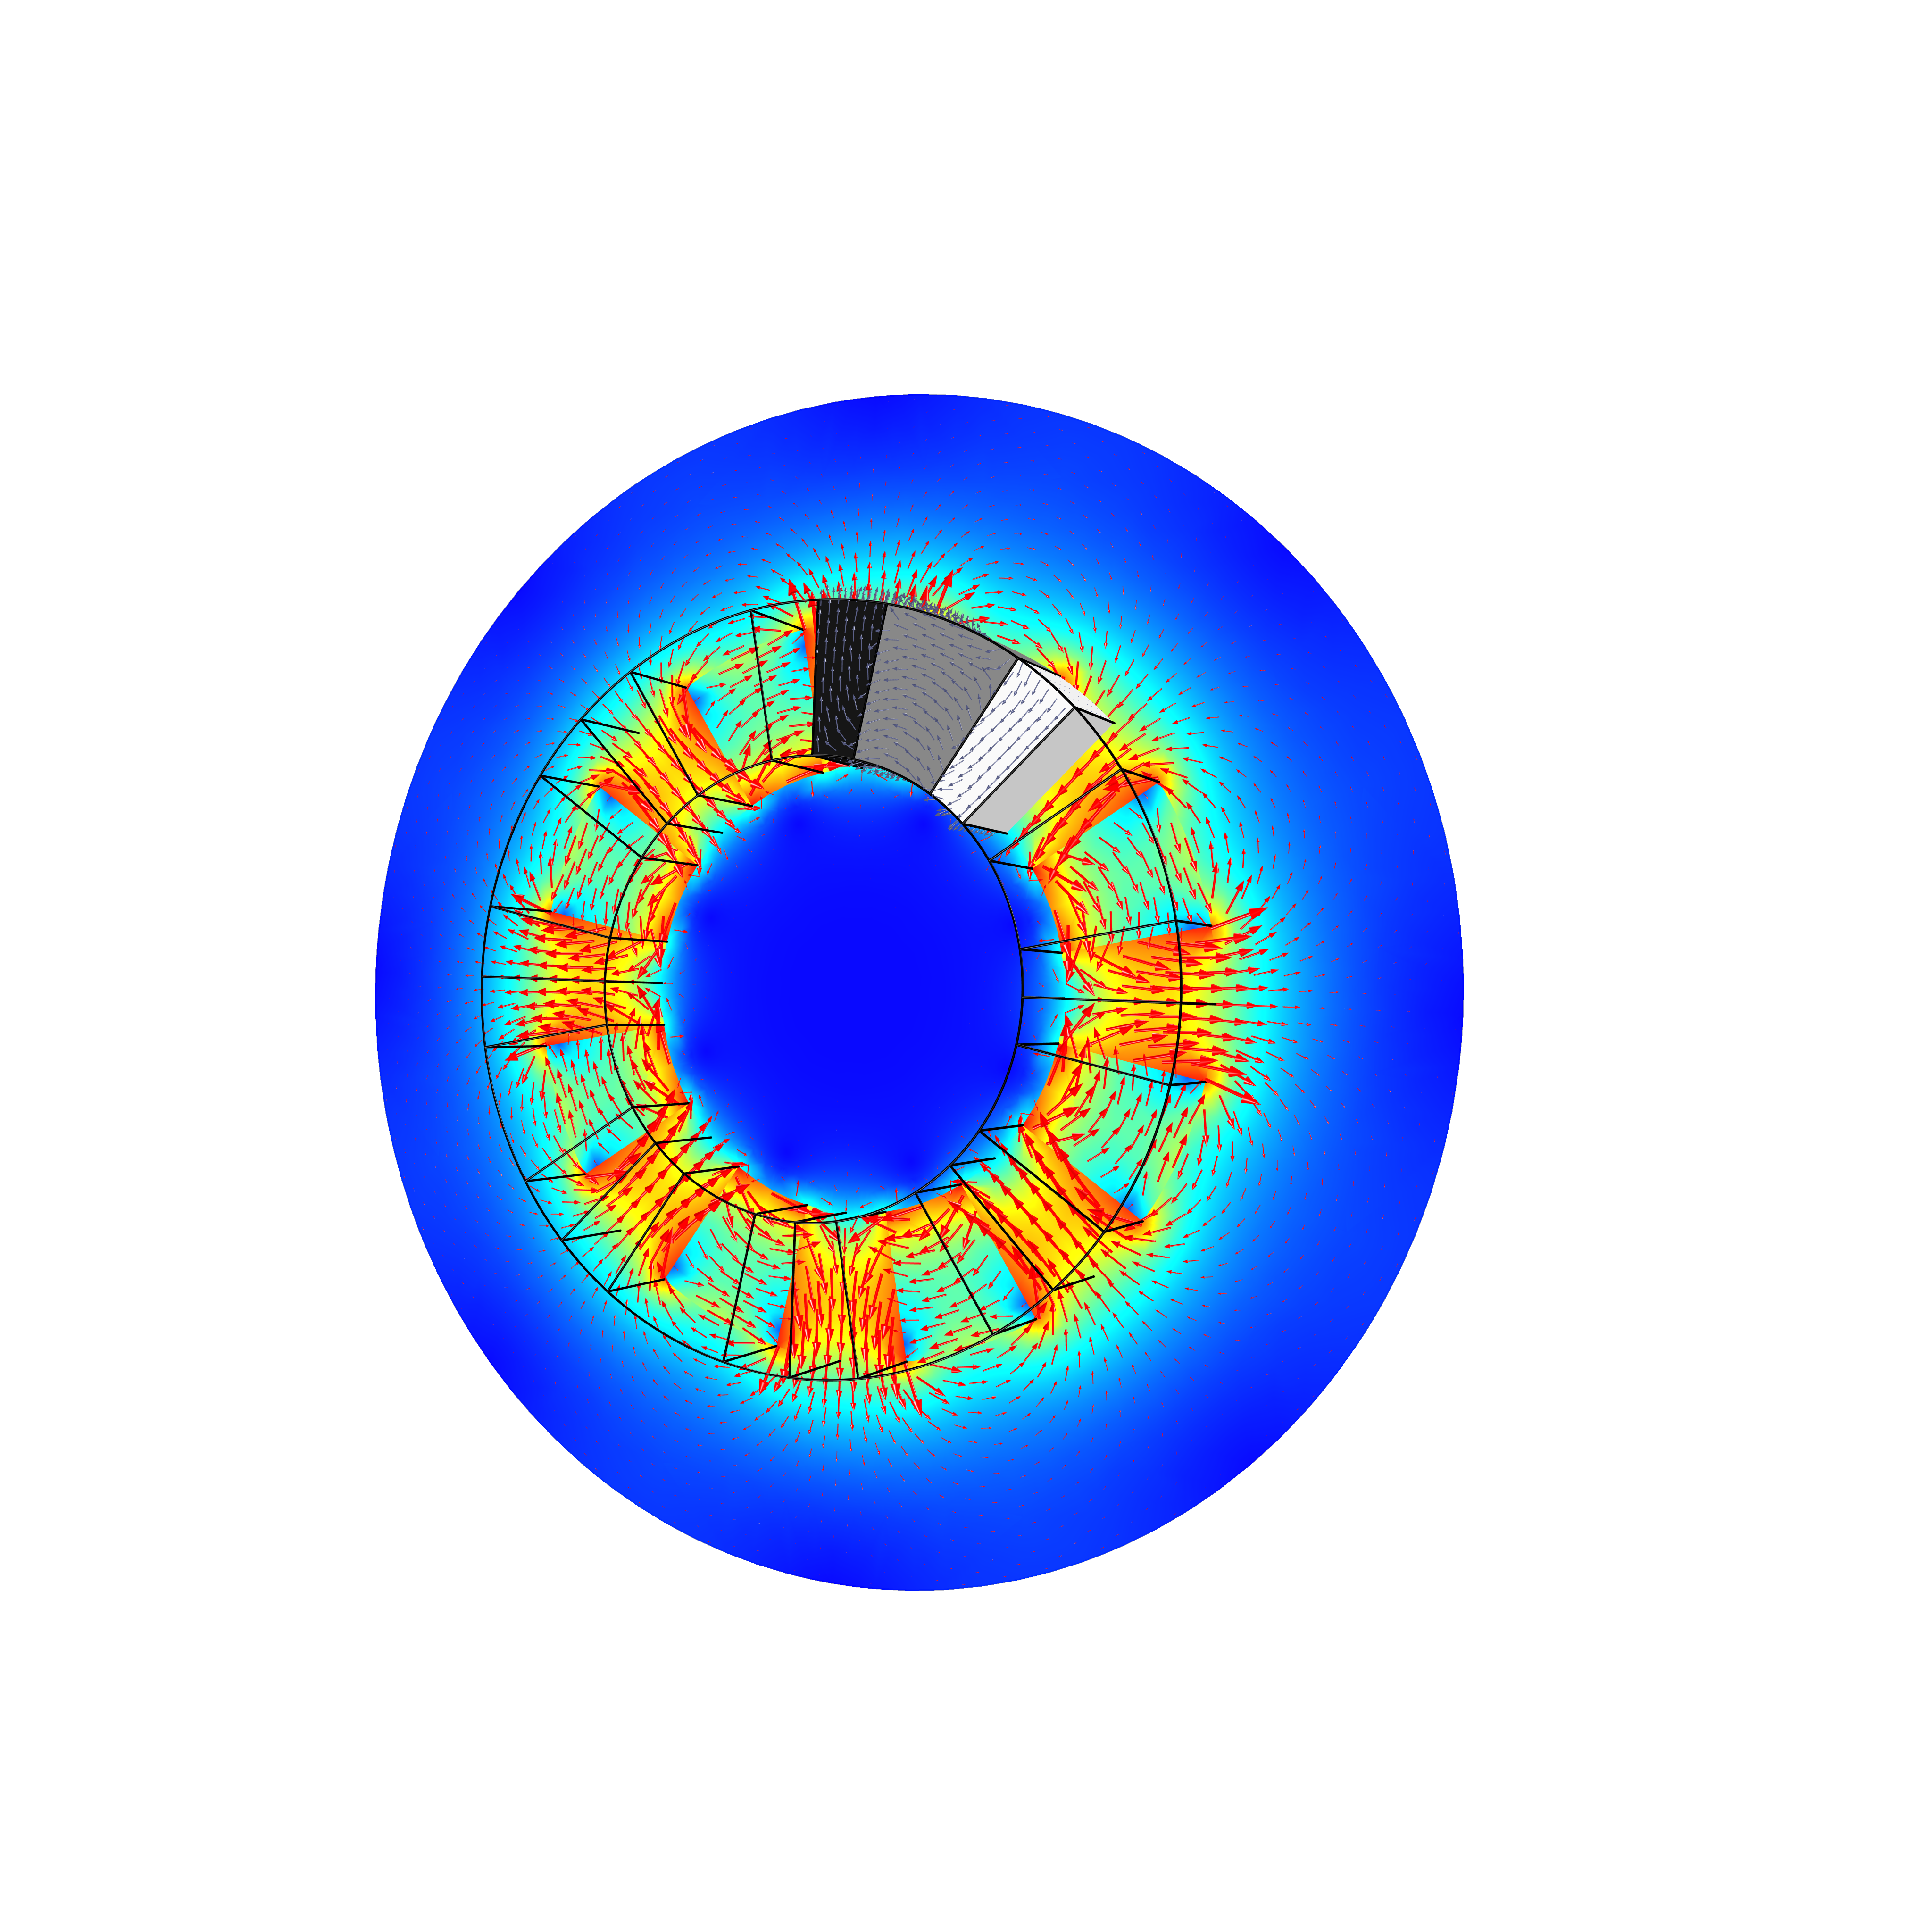
\includegraphics[height=1.5cm]{logo.pdf}}

\begin{document}

\maketitle

\begin{frame}{Table of contents}
    \setbeamertemplate{section in toc}[sections numbered]
    \tableofcontents[hideallsubsections]
\end{frame}

% Introduction %%%%%%%%%%%%%%%%%%%%%%%%%%%%%%%%%%%%%%%%%%%%%%%%%%%%%%%%%%%%%%%%%%%%%%%%%%%%%%%%%%%%%%%%%%%%%%%%%%%%%%%%%%%%%%%
\section{Introduction}

\begin{frame}{Animation}
    \begin{itemize}[<+- | alert@+>]
        \item \alert<4>{This is\only<4>{ really} important}
        \item Now this
        \item And now this
    \end{itemize}
\end{frame}

% Multiple Columns | Blocks %%%%%%%%%%%%%%%%%%%%%%%%%%%%%%%%%%%%%%%%%%%%%%%%%%%%%%%%%%%%%%%%%%%%%%%%%%%%%%%%%%%%%%%%%%%%%%%%%%%
\begin{frame}{Blocks}
    Three different block environments are pre-defined and may be styled with an
    optional background color.

    \begin{columns}[T,onlytextwidth]
        \column{0.5\textwidth}
        \begin{block}{Default}
            Block content.
        \end{block}

        \begin{alertblock}{Alert}
            Block content.
        \end{alertblock}

        \begin{exampleblock}{Example}
            Block content.
        \end{exampleblock}

        \column{0.5\textwidth}

        \metroset{block=fill}

        \begin{block}{Default}
            Block content.
        \end{block}

        \begin{alertblock}{Alert}
            Block content.
        \end{alertblock}

        \begin{exampleblock}{Example}
            Block content.
        \end{exampleblock}

    \end{columns}
\end{frame}

\begin{frame}{References}
    Some references to showcase [allowframebreaks] \cite{knuth92,ConcreteMath,Simpson,Er01,greenwade93}
\end{frame}

% Conclusion %%%%%%%%%%%%%%%%%%%%%%%%%%%%%%%%%%%%%%%%%%%%%%%%%%%%%%%%%%%%%%%%%%%%%%%%%%%%%%%%%%%%%%%%%%%%%%%%%%%%%%%%%%%%%%%%%%
\begin{frame}[standout]
    Questions?
\end{frame}

\appendix

\begin{frame}[allowframebreaks]{References}

    \bibliography{demo}
    \bibliographystyle{abbrv}

\end{frame}

\end{document}